% !TEX program = xelatex
% ¡Recuerda compilar con XeLaTeX o LuaLaTeX!
\documentclass{article}

% --- Cargar nuestro fichero de estilo ---
% Se asume que paper_style.sty está disponible o se usan paquetes estándar.
\usepackage{paper_style}

% --- PAQUETES PARA EL CONTENIDO DEL DOCUMENTO ---
\usepackage{graphicx}
\usepackage{subcaption}
\usepackage{amsmath}
\usepackage{booktabs}
\usepackage{geometry}
\usepackage{hyperref}
\usepackage{enumitem}
\usepackage{float}
\usepackage{soul}
\usepackage{xcolor}


% --- Información del Paper ---
\title{Informe: \\ Práctica 3: Redes Virtuales y Seguridad de Acceso}
\author{
	Jordi Blasco Lozano \\
	\small Infraestructuras y Servicios Cloud \\
	\small Universidad de Alicante
}
\date{\today}

% --- Comienzo del Documento ---
\begin{document}
	
	\maketitle

	\begin{abstract}
	\noindent 
	\end{abstract}
	\begin{figure}[H]
	\centering
	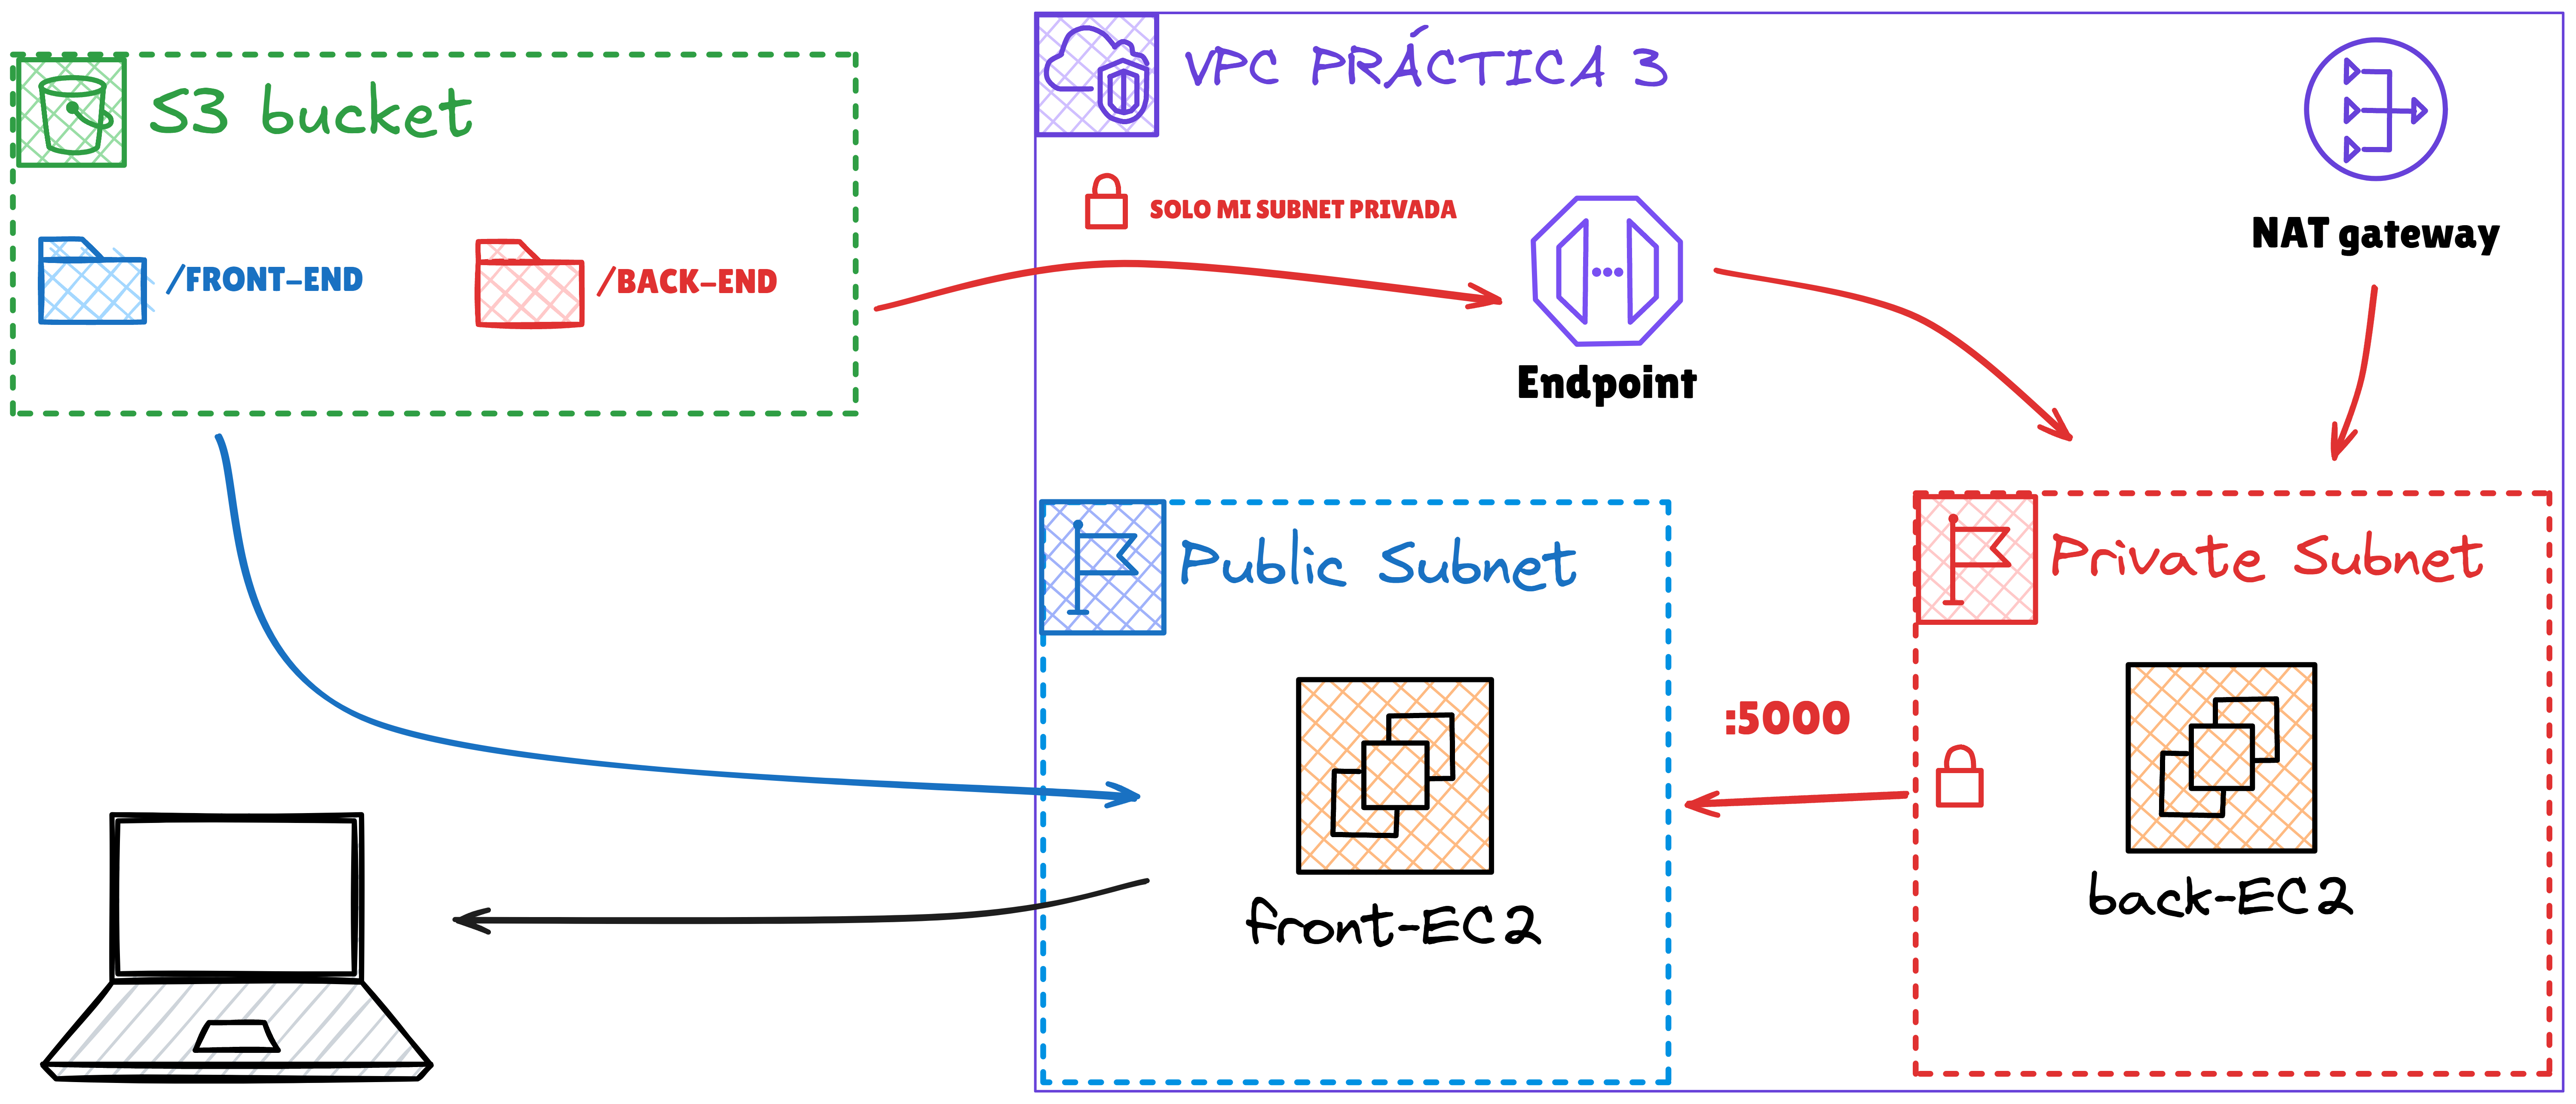
\includegraphics[width=0.95\textwidth]{esquema.png}
	\end{figure}


	\tableofcontents

	\newpage

	\section{Creación de la instancia base}

		
	\subsection{Configuración de red}


\end{document}
